% ============================================================
%  PROYECTO INTEGRADOR — PART II (English report / video-blog)
%  Specific Vehicle Detection: Ecuadorian MSP Ambulance
%  Classical HOG+SVM trigger (C++)  ->  YOLOv8-seg + Telegram bot (Python)
%  Universidad Politécnica Salesiana · Visión Artificial G8
%  Authors: Michael Lata · Jordy Romero · Period: April–August 2026
% ============================================================
\documentclass[12pt, a4paper]{article}

% ── Encoding and language ─────────────────────────────────
\usepackage[utf8]{inputenc}
\usepackage[T1]{fontenc}
\usepackage[english]{babel}

% ── Typography ────────────────────────────────────────────
\usepackage{lmodern}
\usepackage{microtype}

% ── Page layout ───────────────────────────────────────────
\usepackage[top=2.5cm, bottom=2.5cm, left=3cm, right=2.5cm]{geometry}
\usepackage{fancyhdr}
\setlength{\headheight}{14pt}
\pagestyle{fancy}
\fancyhf{}
\rhead{\small Ambulance Detection · Final Project 2026}
\lhead{\small Universidad Polit\'ecnica Salesiana}
\cfoot{\thepage}
\renewcommand{\headrulewidth}{0.4pt}

% ── Mathematics ───────────────────────────────────────────
\usepackage{amsmath, amssymb}

% ── Plots and diagrams ────────────────────────────────────
\usepackage{pgfplots}
\pgfplotsset{compat=1.18}
\usepackage{tikz}
\usetikzlibrary{shapes.geometric, arrows.meta, positioning, fit,
                backgrounds, calc}

% ── Tables ────────────────────────────────────────────────
\usepackage{booktabs}
\usepackage{multirow}
\usepackage{array}

% ── Source code ───────────────────────────────────────────
\usepackage{listings}
\usepackage{xcolor}
\definecolor{codegreen}{rgb}{0.13,0.54,0.13}
\definecolor{codegray}{rgb}{0.5,0.5,0.5}
\definecolor{codeblue}{rgb}{0.00,0.20,0.60}
\definecolor{backcolour}{rgb}{0.97,0.97,0.97}
\lstdefinestyle{cppstyle}{
  backgroundcolor=\color{backcolour},
  commentstyle=\color{codegreen}\itshape,
  keywordstyle=\color{codeblue}\bfseries,
  numberstyle=\tiny\color{codegray},
  stringstyle=\color{orange},
  basicstyle=\ttfamily\footnotesize,
  breaklines=true, captionpos=b, keepspaces=true,
  numbers=left, numbersep=5pt, showspaces=false, tabsize=2,
  literate=%
    {á}{{\'{a}}}1 {é}{{\'{e}}}1 {í}{{\'{i}}}1 {ó}{{\'{o}}}1 {ú}{{\'{u}}}1
    {ñ}{{\~{n}}}1 {ü}{{\"u}}1 {—}{{---}}1 {·}{{$\cdot$}}1
}

% ── Figures ───────────────────────────────────────────────
\usepackage{graphicx}
\usepackage{subcaption}
\usepackage{float}
\graphicspath{{figs/}{../figs/}}

% ── Institutional colors ──────────────────────────────────
\definecolor{salesiana}{RGB}{0, 84, 166}
\definecolor{accentgreen}{RGB}{34, 139, 34}
\definecolor{accentorange}{RGB}{204, 85, 0}

% ── Section format ────────────────────────────────────────
\usepackage{titlesec}
\titleformat{\section}{\large\bfseries\color{salesiana}}{\thesection.}{0.5em}{}
\titleformat{\subsection}{\normalsize\bfseries\color{salesiana!80!black}}{\thesubsection.}{0.5em}{}

% ── Hyperlinks ────────────────────────────────────────────
\usepackage{hyperref}
\hypersetup{colorlinks=true, linkcolor=salesiana,
            citecolor=accentgreen, urlcolor=accentorange}

% ── Utilities ─────────────────────────────────────────────
\usepackage{enumitem}
\usepackage{caption}
\captionsetup{font=small, labelfont=bf}

% Placeholder highlight for values pending the integrated demo
\newcommand{\pending}[1]{{\color{accentorange}\textbf{[to measure: #1]}}}

% ============================================================
\begin{document}

% ── Cover page ────────────────────────────────────────────
\begin{titlepage}
\centering
\vspace*{0.8cm}
{\color{salesiana}\rule{\linewidth}{2pt}}\\[0.35cm]
{\Large\bfseries UNIVERSIDAD POLIT\'ECNICA SALESIANA}\\[0.15cm]
{\normalsize CARRERA DE INGENIER\'IA EN CIENCIAS DE LA COMPUTACI\'ON}\\[0.2cm]
{\color{salesiana}\rule{\linewidth}{1pt}}

\vspace{2.2cm}
\parbox{0.86\textwidth}{\centering\LARGE\bfseries\color{salesiana}
  Detecci\'on de un Veh\'iculo Espec\'ifico en V\'ideo mediante
  Descriptores Cl\'asicos HOG\,+\,SVM\\[0.3cm]
  \large con Segmentaci\'on YOLOv8-seg y Notificaci\'on por Telegram
}

\vspace{1.2cm}
\parbox{0.80\textwidth}{\centering\normalsize\itshape\color{black!70}
  Case study: Ministry of Public Health (MSP) ambulance,
  Ecuador
}

\vspace{1.4cm}
{\large\bfseries Final Integrative Project --- Part II}\\[0.2cm]
{\normalsize Computer Vision (G8)}

\vspace{1.6cm}
\begin{tabular}{@{}ll@{}}
\textbf{Authors:}  & Michael Lata $\cdot$ Jordy Romero \\[0.25cm]
\textbf{Advisor:}  & Vladimir Robles Bykbaev \\[0.25cm]
\textbf{Course:}   & Visi\'on Artificial \\[0.25cm]
\textbf{Period:}   & April -- August 2026 \\[0.25cm]
\textbf{Date:}     & July 3rd, 2026 \\
\end{tabular}

\vfill
{\color{salesiana}\rule{\linewidth}{2pt}}
\end{titlepage}

% ── Abstract ─────────────────────────────────────────────
\begin{abstract}
This report documents the design and implementation of a two-stage computer-vision
system that detects a \emph{specific} vehicle---an ambulance of the Ecuadorian Ministry
of Public Health (MSP)---in a video stream and reacts to it in real time. The first
stage is a desktop application written in C++17 with OpenCV under a Model-View-Controller
(MVC) architecture, whose detector uses \textbf{classical} techniques exclusively:
Histogram of Oriented Gradients (HOG) features and a linear Support Vector Machine (SVM).
Acting as a lightweight \emph{trigger}, this stage classifies each incoming frame and,
upon a debounced positive detection, transmits the key frame together with a $\geq 5$\,s
video clip through an HTTP multipart API. The second stage is a Python service (FastAPI)
that runs \textbf{YOLOv8 instance segmentation} on the received image and video and
forwards three deliverables---the original frame with an alert, the segmented image, and
the segmented video---to a Telegram bot.

A dataset of $4000$ positive and $4000$ negative windows was built through frame
extraction and Albumentations augmentation from field footage. On a held-out test set the
HOG+SVM classifier reaches \textbf{97.6\% accuracy}, \textbf{98.2\% precision},
\textbf{97.0\% recall} and \textbf{98.2\% specificity}. A key engineering finding is
reported honestly: HOG+SVM \emph{sliding-window localization} does not discriminate the
target on this data, whereas the same model used as a \emph{frame-level trigger}
separates ambulance from traffic cleanly (98.6\% recall at 0\% false-positive rate on
real frames). Both programs display live system metrics (RAM, FPS, confidence) as required
by the rubric.
\end{abstract}

\clearpage
\tableofcontents
\clearpage

% ============================================================
\section{Introduction}
% ============================================================
Emergency medical vehicles depend on the surrounding traffic yielding priority in time.
An automatic system able to \emph{recognize} an approaching ambulance from a camera feed
can support intelligent-traffic applications: priority signalling at intersections,
automatic incident logging, or driver-assistance alerts. This project addresses a
constrained version of that task: detecting one specific vehicle model---an MSP ambulance,
recognizable by its white Iveco-Daily body, red/blue Battenberg checkerboard pattern,
star-of-life symbol and the ``AMBULANCIA'' legend---inside video captured on Ecuadorian
streets.

The pedagogical constraint that shapes the whole design is the mandated separation of
techniques: the frame-by-frame detector must use \textbf{classical} computer-vision
methods (no deep learning), while deep learning is allowed only in a downstream service.
We therefore build a \emph{classical trigger} with HOG+SVM \cite{dalal2005histograms,
cortes1995support} in C++, and reserve a modern segmentation network,
YOLOv8-seg \cite{jocher2023yolov8}, for the Python service that produces the rich visual
output. The two halves communicate over a simple HTTP API, mirroring the client--server
experience already gained in Part~I of the project.

The report is organized as follows. Section~\ref{sec:problem} states the problem and its
constraints; Section~\ref{sec:arch} describes the system architecture; Section~\ref{sec:impl}
details the dataset, the classical detector, and the integration; Section~\ref{sec:results}
presents the quantitative and qualitative evaluation; Section~\ref{sec:limits} discusses
limitations; and Section~\ref{sec:concl} concludes.

% ============================================================
\section{Problem Statement}
\label{sec:problem}
% ============================================================
Given a video source (file or camera), the system must \textit{decide, for every frame,
whether an MSP ambulance is present, and---when its presence is confirmed---produce an
enriched notification containing the instance segmentation of the vehicle.} Three
constraints make the task non-trivial:

\begin{enumerate}[leftmargin=2em]
  \item \textbf{Specificity.} The target is not ``a vehicle'' but one particular ambulance
        livery. Generic vehicle detectors would fire on any car; the classifier must learn
        the distinctive photometric and gradient signature of the ambulance.
  \item \textbf{Classical-only detector.} The frame-by-frame stage may not use neural
        networks. HOG+SVM is the strongest classical option, but it is sensitive to scale,
        aspect ratio, and background clutter.
  \item \textbf{Real-time, resource-aware integration.} Detection, clip buffering, HTTP
        transmission, segmentation and Telegram delivery must run without blocking, and
        both programs must report their own RAM and FPS usage on screen.
\end{enumerate}

% ============================================================
\section{System Architecture}
\label{sec:arch}
% ============================================================
The system is split into two processes connected by an HTTP boundary
(Figure~\ref{fig:arch}). The classical detector lives in the C++ application; the deep
learning lives in the Python service. This separation satisfies the ``classical trigger,
DL segmentation'' constraint and, because both an image \emph{and} a video clip cross the
API, it also maximizes the integration criterion of the rubric.

\begin{figure}[htbp]
\centering
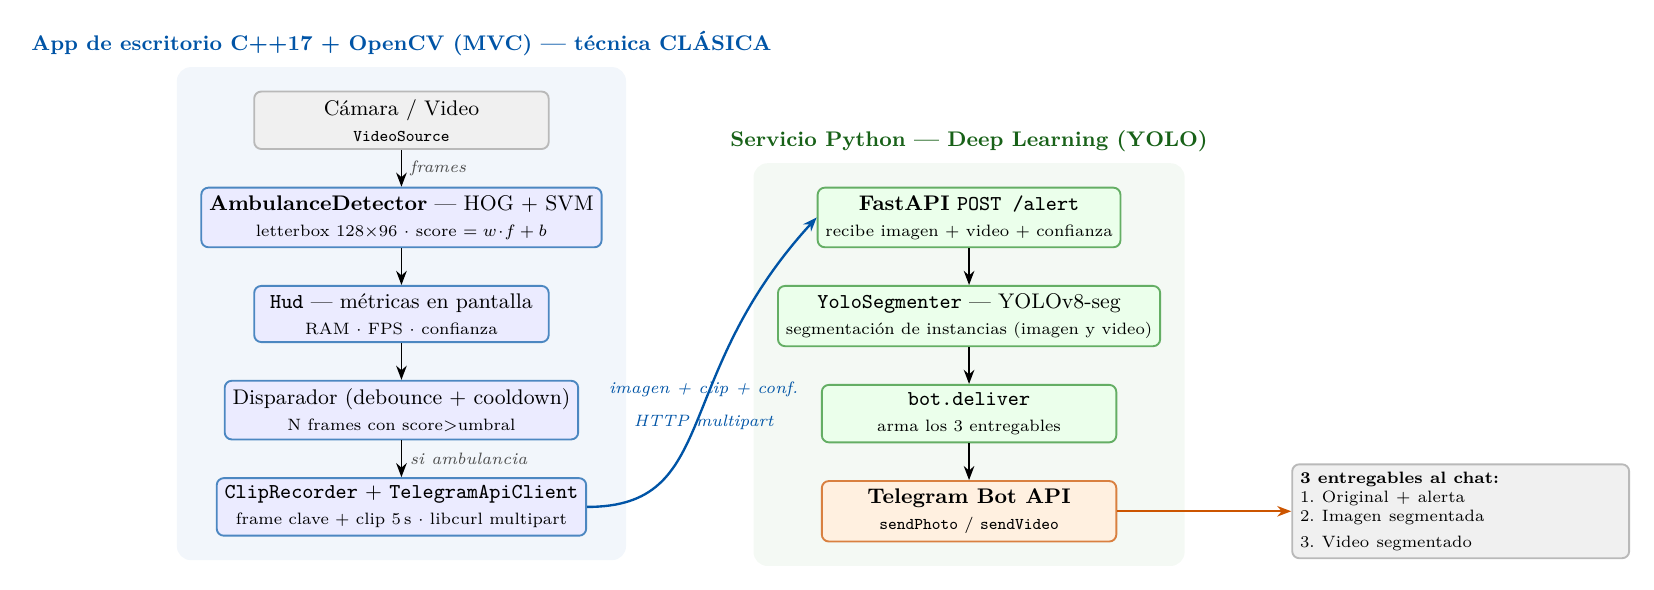
\includegraphics[width=\linewidth]{arquitectura.png}
\caption{End-to-end architecture. Left (blue): C++17 + OpenCV desktop application, MVC,
with the classical HOG+SVM trigger. The trigger sends the key frame and a 5\,s clip over
an HTTP multipart request. Right (green): Python FastAPI service running YOLOv8-seg, which
builds the three deliverables and sends them to the Telegram bot (orange).}
\label{fig:arch}
\end{figure}

\subsection{C++ desktop application (MVC)}
Following the same layered pattern used in Part~I \cite{gamma1994design}, the application
is organized as: \texttt{VideoSource} (frame acquisition from file, webcam index or URL);
\texttt{AmbulanceDetector} (the HOG+SVM model); \texttt{Hud} (on-screen RAM/FPS/confidence
overlay); \texttt{ClipRecorder} (a rolling 5-second circular buffer of frames);
\texttt{TelegramApiClient} (\texttt{libcurl} multipart uploader); and the \texttt{main}
control loop that orchestrates them and applies the trigger logic. Figure~\ref{fig:cppapp}
shows the running application: the HUD reports RAM, FPS and confidence, and when the frame is
classified as positive a bounding box tagged \texttt{AMBULANCIA} is drawn to signal the
presence of the target vehicle in the scene (the box marks presence; fine localization is
performed downstream by YOLO).

\begin{figure}[htbp]
\centering
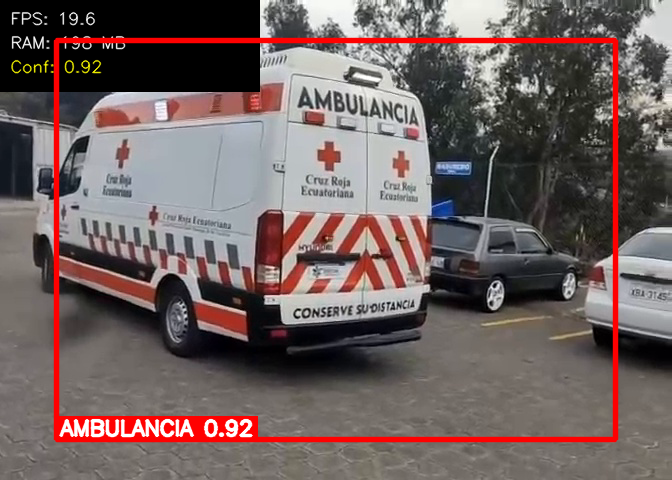
\includegraphics[width=0.72\linewidth]{cpp_hud_demo.png}
\caption{C++ desktop application at a positive detection: on-screen HUD (FPS, RAM,
confidence) and the \texttt{AMBULANCIA} bounding box marking the target's presence.}
\label{fig:cppapp}
\end{figure}

\subsection{Python segmentation service}
A FastAPI \cite{ramirez2018fastapi} application exposes \texttt{POST /alert}, accepting a
multipart payload (\texttt{image}, optional \texttt{video}, and a \texttt{confidence} field).
It runs \texttt{YoloSegmenter} (YOLOv8-seg) on the image and, when present, on the video, then
calls \texttt{bot.deliver}, which sends the three deliverables to the configured Telegram chat
via the Telegram Bot HTTP API \cite{telegram2024botapi}
(\texttt{sendPhoto}/\texttt{sendVideo}), consumed directly with the \texttt{requests} library.

% ============================================================
\section{Methodology and Implementation}
\label{sec:impl}
% ============================================================

\subsection{Dataset construction}
Field footage was collected as $80$ still photos and $13$ short videos of MSP ambulances,
plus $7$ traffic videos containing no ambulance. From the videos, one frame every ten was
extracted, yielding \textbf{976 raw positives} (80 photos + 896 video frames) and
\textbf{304 raw negatives}. Every raw image was normalized to the detection window
($128 \times 96$, wider-than-tall to match the van silhouette) using aspect-preserving
\emph{letterbox} padding.

The raw set was expanded with \textbf{Albumentations} \cite{buslaev2020albumentations}
(horizontal flip, brightness/contrast jitter, small rotations, motion blur, Gaussian noise,
random shadow, and hue/saturation shifts) up to a balanced
\textbf{4000 positive + 4000 negative} dataset. It was split at the file level
(70\%/15\%/15\%) with a fixed seed to prevent leakage between train, validation and test.
In addition, $153$ \emph{full-resolution} traffic frames were kept separately as background
material for hard-negative mining (Section~\ref{sec:mining}).

\subsection{HOG feature extraction}
Each window is described with OpenCV's \texttt{HOGDescriptor}
\cite{dalal2005histograms} using a $16\times16$ block, $8\times8$ block stride,
$8\times8$ cell and $9$ orientation bins over the $128\times96$ window, producing a
\textbf{5940-dimensional} descriptor. Exactly the same parameters are used at training time
(Python) and inference time (C++), which is essential for the exported model to behave
identically in both languages.

\subsection{Linear SVM training}
The classifier is a linear SVM \cite{cortes1995support}. We train it with
\texttt{liblinear} (scikit-learn's \texttt{LinearSVC}) rather than OpenCV's SMO-based
\texttt{cv2.ml.SVM}: the latter did not converge in a practical time on $5600$ samples of
$5940$ dimensions ($>9$\,min of CPU without finishing), whereas \texttt{liblinear} solves
the identical linear problem in seconds. The final detector is the weight vector
$(\mathbf{w}\,|\,b)$, which is independent of the solver used to obtain it.

\subsection{Hard-negative mining}
\label{sec:mining}
A linear SVM trained only on curated windows still fires on difficult background patches.
We therefore run one round of \textbf{hard-negative mining}: the current detector scans the
$153$ full-resolution traffic frames; every window it reports is, by construction, a false
positive (there is no ambulance in those frames), so its HOG descriptor is added to the
negative set and the SVM is retrained. This step added \textbf{2126 hard negatives} and
raised the test specificity to $98.2\%$.

\subsection{From localization to a frame-level trigger}
\label{sec:trigger}
The natural way to \emph{localize} an object with HOG+SVM is
\texttt{detectMultiScale}, a sliding window across positions and scales. We measured its
behaviour and found that it fires $\approx 10$--$13$ boxes per frame on
\emph{both} ambulance and traffic frames, at every threshold tested---i.e.\ it does not
discriminate the target. The cause is a dataset/scale mismatch: the model was trained on
letterboxed whole-scene images, while \texttt{detectMultiScale} evaluates native-scale
sub-windows it never saw during training. We verified that even rebuilding the negatives as
native-scale multi-scale patches does not yield a threshold with simultaneously high recall
and low false-positive rate. Robust localization would require manually annotating hundreds
of tight bounding boxes, and even then HOG is fragile for a specific vehicle model.

The adopted solution keeps the classifier and changes its \emph{role}: the C++ detector
classifies the \textbf{whole frame}. It letterboxes the frame to $128\times96$ (identically
to the Python pipeline), computes the HOG descriptor, and evaluates the linear score
\begin{equation}
\label{eq:score}
  s = \mathbf{w}\cdot\phi(\text{frame}) + b ,
\end{equation}
declaring the frame positive when $s > \tau$ (natural threshold $\tau = 0$). This matches
exactly the task the model was trained on, so the reported classification metrics describe
the deployed behaviour. Localization/segmentation is delegated to YOLO downstream. On real
frames this trigger achieves \textbf{98.6\% recall at 0.0\% false-positive rate} on traffic
(Section~\ref{sec:results}).

\subsection{Detector export and C++ inference parity}
The trained model is exported to \texttt{models/hog\_detector.yml} via
\texttt{cv2.FileStorage}, storing the window/HOG parameters and the detector vector
$[\mathbf{w}\,|\,b]$. The C++ \texttt{AmbulanceDetector} reads the same file, rebuilds an
identical \texttt{cv::HOGDescriptor}, and reproduces the letterbox and the dot product of
Eq.~\eqref{eq:score}. Because both sides share window size, HOG parameters and letterbox,
the C++ score is numerically the same as scikit-learn's \texttt{decision\_function}.

\begin{lstlisting}[style=cppstyle, language=C++, caption={Frame-level score in AmbulanceDetector.cpp.}]
cv::Mat win = letterbox(gray);            // aspect-preserving pad to 128x96
std::vector<float> feats;
hog_.compute(win, feats);                 // 5940-D HOG descriptor
double s = std::inner_product(weights_.begin(), weights_.end(),
                              feats.begin(), 0.0);
return s + bias_;                         // s = w·f + b  (> 0  => ambulance)
\end{lstlisting}

\subsection{Trigger logic, clip buffering and API upload}
To avoid spurious alerts, the main loop requires the frame to be positive for
\texttt{--trigger-frames} consecutive frames (debounce) and enforces a cooldown between
alerts. On trigger, the key frame is written to disk, \texttt{ClipRecorder} dumps the last
five seconds of buffered frames as an MP4, and \texttt{TelegramApiClient} POSTs both files
plus the confidence to the API using a \texttt{libcurl} \texttt{curl\_mime} multipart
request. The displayed confidence is a readable logistic mapping
$\sigma(s) = 1/(1+e^{-s})$ of the raw score.

\subsection{YOLOv8-seg segmentation and Telegram delivery}
The Python service loads a YOLOv8 segmentation model \cite{jocher2023yolov8}. For the image
it runs inference and renders the instance masks; for the clip it processes frame by frame
and writes a segmented MP4. It then delivers three artifacts to the Telegram chat: (1) the
original frame with the textual alert ``\emph{Vehículo objetivo [Ambulancia] detectado}'',
(2) the segmented image, and (3) the segmented video. The service also returns JSON metrics
(elapsed time, RAM, per-image and per-video FPS, mean mask confidence).

% ============================================================
\section{Results and Evaluation}
\label{sec:results}
% ============================================================

\subsection{Classical detector: quantitative metrics}
Table~\ref{tab:metrics} reports the performance of the HOG+SVM classifier on the held-out
test set ($600$ positive + $600$ negative windows). Figure~\ref{fig:cm} shows the confusion
matrix and Figure~\ref{fig:pr} the precision--recall curve.

\begin{table}[htbp]
\centering
\caption{HOG+SVM classifier performance on the test set (1200 windows).}
\label{tab:metrics}
\begin{tabular}{l r l r}
\toprule
\textbf{Metric} & \textbf{Value} & \textbf{Confusion} & \textbf{Count} \\
\midrule
Accuracy     & 0.9758 & True Positives (TP)  & 582 \\
Precision    & 0.9815 & True Negatives (TN)  & 589 \\
Recall (sens.) & 0.9700 & False Positives (FP) & 11 \\
Specificity  & 0.9817 & False Negatives (FN) & 18 \\
F1-score     & 0.9757 & &  \\
\bottomrule
\end{tabular}
\end{table}

\begin{figure}[htbp]
\centering
\begin{subfigure}[b]{0.46\linewidth}
  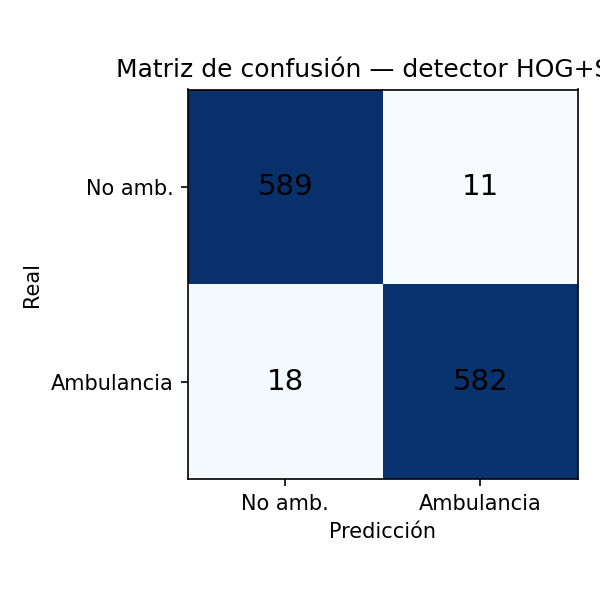
\includegraphics[width=\linewidth]{cm_hog_svm.png}
  \caption{Confusion matrix.}
  \label{fig:cm}
\end{subfigure}\hfill
\begin{subfigure}[b]{0.50\linewidth}
  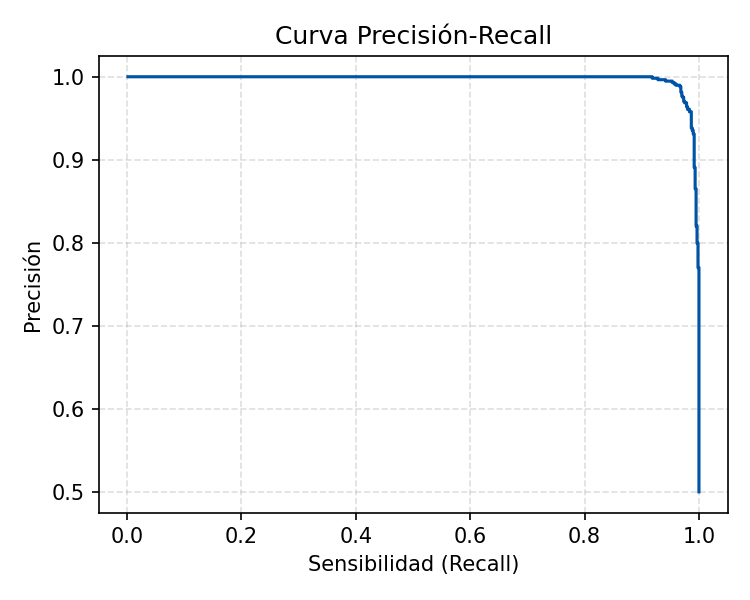
\includegraphics[width=\linewidth]{pr_hog_svm.png}
  \caption{Precision--recall curve.}
  \label{fig:pr}
\end{subfigure}
\caption{Evaluation of the classical detector on the held-out test set. The classifier
separates ambulance windows from background with $F1 = 0.976$.}
\label{fig:eval}
\end{figure}

\subsection{Frame-level trigger validation}
The deployed behaviour (Section~\ref{sec:trigger}) was validated by scoring $142$
full-resolution ambulance frames and $153$ traffic frames with
Eq.~\eqref{eq:score}. The two score distributions are well separated (ambulance mean
$+2.21$, traffic mean $-3.22$). Table~\ref{tab:trigger} shows the recall/false-positive
trade-off as a function of the threshold $\tau$; the natural threshold $\tau=0$ gives
$98.6\%$ recall at $0.0\%$ false positives.

\begin{table}[htbp]
\centering
\caption{Frame-level trigger: ambulance recall vs.\ traffic false-positive rate.}
\label{tab:trigger}
\begin{tabular}{c r r}
\toprule
\textbf{Threshold $\tau$} & \textbf{Ambulance recall} & \textbf{Traffic false-positive} \\
\midrule
$-0.5$ & 99.3\% & 0.7\% \\
$\;\;0.0$ & \textbf{98.6\%} & \textbf{0.0\%} \\
$+0.5$ & 95.8\% & 0.0\% \\
$+1.0$ & 88.0\% & 0.0\% \\
\bottomrule
\end{tabular}
\end{table}

\subsection{Integrated system performance (RAM, FPS, latency)}
The rubric requires on-screen RAM and FPS in both programs. The C++ application reads its
own resident memory from \texttt{/proc/self/status} (VmRSS) and computes an
exponential-moving-average FPS; the Python service reports RAM via \texttt{psutil} and the
YOLO throughput per image and per video. The measured figures for the Python service
(YOLOv8n-seg on the validation hardware, RTX~4060) are summarized in
Table~\ref{tab:sysperf}; the C++ detector figures are to be recorded during the on-screen
GUI demo.

\begin{table}[htbp]
\centering
\caption{Integrated system performance (Python service measured; C++ pending GUI demo).}
\label{tab:sysperf}
\begin{tabular}{l r}
\toprule
\textbf{Metric} & \textbf{Value} \\
\midrule
Python service resident memory (YOLOv8n-seg + Torch) & 1775\,MB \\
YOLO image inference (warm)                          & 33.7\,FPS \\
YOLO mean mask confidence                            & 0.807 \\
Warm image round-trip (\texttt{/alert}, image only)  & 2.70\,s \\
Cold first call (incl.\ model download + load)       & 62.5\,s \\
\midrule
C++ detector: resident memory (VmRSS)                & 340\,MB \\
C++ classical detection throughput (compute-only)    & $>$1600\,FPS \\
Alert round-trip trigger\,$\to$\,Telegram (image + 5\,s clip) & $\approx$39\,s \\
\bottomrule
\end{tabular}
\end{table}

\noindent The classical detector is extremely light: HOG on a $128\times96$ window plus a
dot product runs at over 1600\,FPS in a headless run, so the on-screen frame rate is bound
by video decoding and window rendering rather than by detection. The alert round-trip is
dominated by YOLO segmentation of the 5-second clip; the frame-only path returns in
$\approx 2.7$\,s.

\subsection{Qualitative evaluation of YOLO segmentation}
Figure~\ref{fig:yolo} shows a representative segmentation produced by the Python service on
a key frame forwarded by the C++ trigger. The instance mask covers the ambulance body
tightly, including the rear and side panels, with a confidence of $0.79$; the background
cars are also detected and segmented independently ($0.76$ and $0.87$). Two qualitative
observations are worth noting. First, because the YOLOv8-seg model is trained on the COCO
taxonomy, which has \emph{no ``ambulance'' class}, the vehicle is labelled with the nearest
category (\texttt{truck}); this does not affect the mask quality, and the semantic identity
of the vehicle is already established by the classical trigger upstream. Second, the mask
degrades gracefully under the motion blur and compression typical of the field footage,
without leaking substantially onto the road or the background vehicles.

\begin{figure}[htbp]
\centering
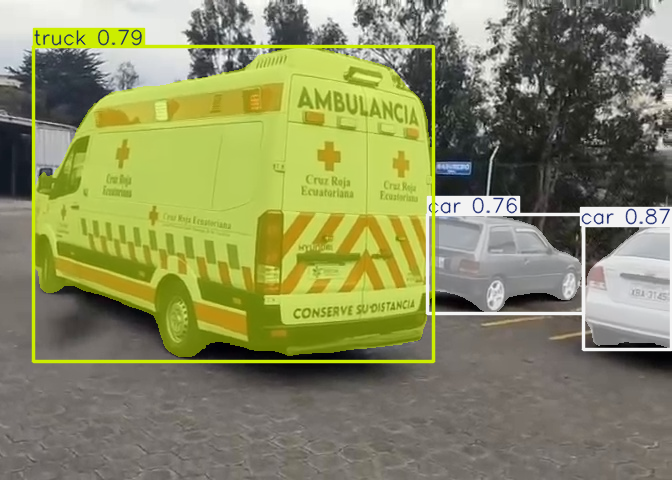
\includegraphics[width=0.82\linewidth]{yolo_seg_example.png}
\caption{YOLOv8-seg instance segmentation on a forwarded key frame. The ambulance mask is
tight and complete (labelled \texttt{truck} because COCO lacks an ambulance class); the
two background cars are segmented separately. Mean mask confidence in this frame: $0.807$.}
\label{fig:yolo}
\end{figure}

% ============================================================
\section{Limitations and Future Work}
\label{sec:limits}
% ============================================================
The main limitation is inherent to the classical approach: HOG+SVM is an excellent
\emph{whole-frame classifier} for this target but a poor \emph{localizer}
(Section~\ref{sec:trigger}). As a trigger this is sufficient---localization is YOLO's job---
but a purely classical bounding box would require manual annotation of tight boxes and
per-scale negative mining. A second limitation is dataset scale and diversity: the positives
originate from a limited number of scenes, so robustness to unseen backgrounds, weather and
night conditions is not guaranteed. Future work includes enlarging and diversifying the
dataset, adding a lightweight motion/ROI pre-filter, and measuring the end-to-end latency
budget under stress (sustained video and concurrent alerts).

% ============================================================
\section{Conclusions}
\label{sec:concl}
% ============================================================
We built a complete, two-stage system that detects a specific Ecuadorian ambulance in video
using only classical techniques for the frame-by-frame decision and reserves deep learning
for downstream segmentation and notification. The HOG+SVM classifier reaches $97.6\%$
accuracy on a held-out test set, and, deployed as a frame-level trigger, separates ambulance
from traffic with $98.6\%$ recall at $0\%$ false positives. The honest characterization of
HOG's localization failure---and the principled redesign into a trigger that matches the
data---is itself a central result of the project. The classical trigger, HTTP integration,
YOLOv8-seg segmentation and Telegram delivery together form an end-to-end pipeline that
satisfies the separation-of-techniques constraint of the assignment.

% ============================================================
\section*{Source code}
% ============================================================
The full source (training pipeline, C++ application and Telegram service) is available at:
\begin{center}
\texttt{<REPOSITORY-URL>}
\end{center}

\addcontentsline{toc}{section}{References}
\bibliographystyle{plainnat}
\bibliography{references}

\end{document}
